% master: main
% format: latex

%%--------------------------------------------------------------------------
\part{Mathematical Equations, Figures and Tables}
%%--------------------------------------------------------------------------

In a thesis, one may need to write many more equations than simple in-text
formula and display formula. In this part, some more involved
formula are included and they will be put in the equation like environments.
The user should also pay attention to the way the equations being numbered,
labeled and cross-referenced.


%%--------------------------------------------------------------------------
\chapter{EQUATIONS AND EQUATION ARRAYS}
%%--------------------------------------------------------------------------

The following equation (\ref{eq:1}) is in the \textbf{equation}
environment and it is labeled,

\begin{equation}
\sqrt{1+\sqrt{1+\sqrt{1+\sqrt{1+\sqrt{1+\sqrt{1+\sqrt{1+x}}}}}}}
 = ? \label{eq:1}
\end{equation}

\LaTeX\ numbers the equation  as long as it is in the equation
or eqnarray environment. The following is an un-labeled equation,
\LaTeX\ still numbers it

\ifAMS
\begin{equation}
    A=
    \begin{pmatrix}
	    a_{11}&a_{12}&\ldots&a_{1n}\\
	     a_{21}&a_{22}&\ldots&a_{2n}\\
	     \vdots&\vdots&\ddots&\vdots\\
	     a_{m1}&a_{m2}&\ldots&a_{mn}
    \end{pmatrix}
\end{equation}
\else
\begin{equation}
    A=
    \left(
    \begin{array}{cccc}
	    a_{11}&a_{12}&\ldots&a_{1n}\\
	     a_{21}&a_{22}&\ldots&a_{2n}\\
	     \vdots&\vdots&\ddots&\vdots\\
	     a_{m1}&a_{m2}&\ldots&a_{mn}
    \end{array}
    \right)
\end{equation}
\fi

If one does not need to number and label a equation, he can place it
inside the math display environment or delimiters, i.e., \textbf{displaymath}
environment and
\begin{verbatim}
\[ ... \]
\end{verbatim}
or
\begin{verbatim}
$$ ... $$
\end{verbatim}
delimiter pairs, e.g.,

$$
\left(\frac{\partial^2}{\partial x^2}+
\frac{\partial^2}{\partial y^2}\right)\left|\varphi(x+iy)\right|^2 = 0
$$

and

\begin{displaymath}
    2\uparrow\uparrow k\mathrel{\mathop=^{\rm def}}
    2^{2^{2^{\cdot^{\cdot^{\cdot^2}}}}}
    \vbox{\hbox{$\Bigr\}\scriptstyle k$}\kern0pt}
\end{displaymath}

or

\[
\prod_{j\ge0}\left(\sum_{k\ge0}a_{jk}z^k\right)
   =\sum_{n\ge0}z^n\,\left(\sum_
    {\stackrel{\scriptstyle k_0,k_1,\ldots\ge0}
    {\scriptstyle k_0+k_1+\cdots=n}}
    a_{0k_0}a_{1k_1}\ldots\,\right)
\]

If there are more than one  equation in a group or there are many lines
in an equation, one can use the \textbf{eqnarray} environment, but he should
pay special attention to those multi-line equations (otherwise all the lines
will be numbered) by using \textbf{nonumber} command  as shown below,

\begin{eqnarray}
 \left(\int_{-\infty}^\infty e^{-x^2}\,dx\right)^2
 & =& \int_{-\infty}^\infty\int_{-\infty}^\infty
   e^{-(x^2+y^2)}\,dx\,dy \nonumber \\
 & =& \int_0^{2\pi}\int_0^\infty e^{-r^2}r\,dr\,d\theta \nonumber \\
 & =& \int_0^{2\pi}\left(\left. -\frac{e^{-r^2}}{2}
   \right|_{r=0}^{\infty}\,\right)\,d\theta \nonumber \\
 & =& \pi
\end{eqnarray}

otherwise

\begin{eqnarray}
\textstyle\sin18^\circ={\frac{1}{4}}(\sqrt5-1)\\
k=1.38\times10^{-23}\rm\,J/^\circ K.
\end{eqnarray}

%%--------------------------------------------------------------------------
\chapter{FIGURES AND TABLES}
%%--------------------------------------------------------------------------
Figures and tables are essential ingredients in a non-trivial engineering or
science thesis. Before the computer typesetting became good enough, these
things took authors lots of time to hand-draw. Nowadays, the computer seems
to be able to draw any kind of simple and fancy figures and tables. Many
users are still computer-generating figures and tables separately from
typesetting the thesis, and then cut-and-paste. However, with good
packages such as \TeX/\LaTeX, one can avoid this type of waste most of times.

In the following, we will see how the figures can be inserted into the
thesis. The figure itself is generated otherwise, and the table is produced
by \LaTeX\ commands.

\section{Figures--Inserting, Captioning and Importing}

Shown in Figure~\ref{fig:1} is a figure (Pitt Engineering Thesis Guide
Manual has a good definition as for what is called a figure).  This Figure
is generated by:
\begin{verbatim}
\begin{figure}
    \centering
    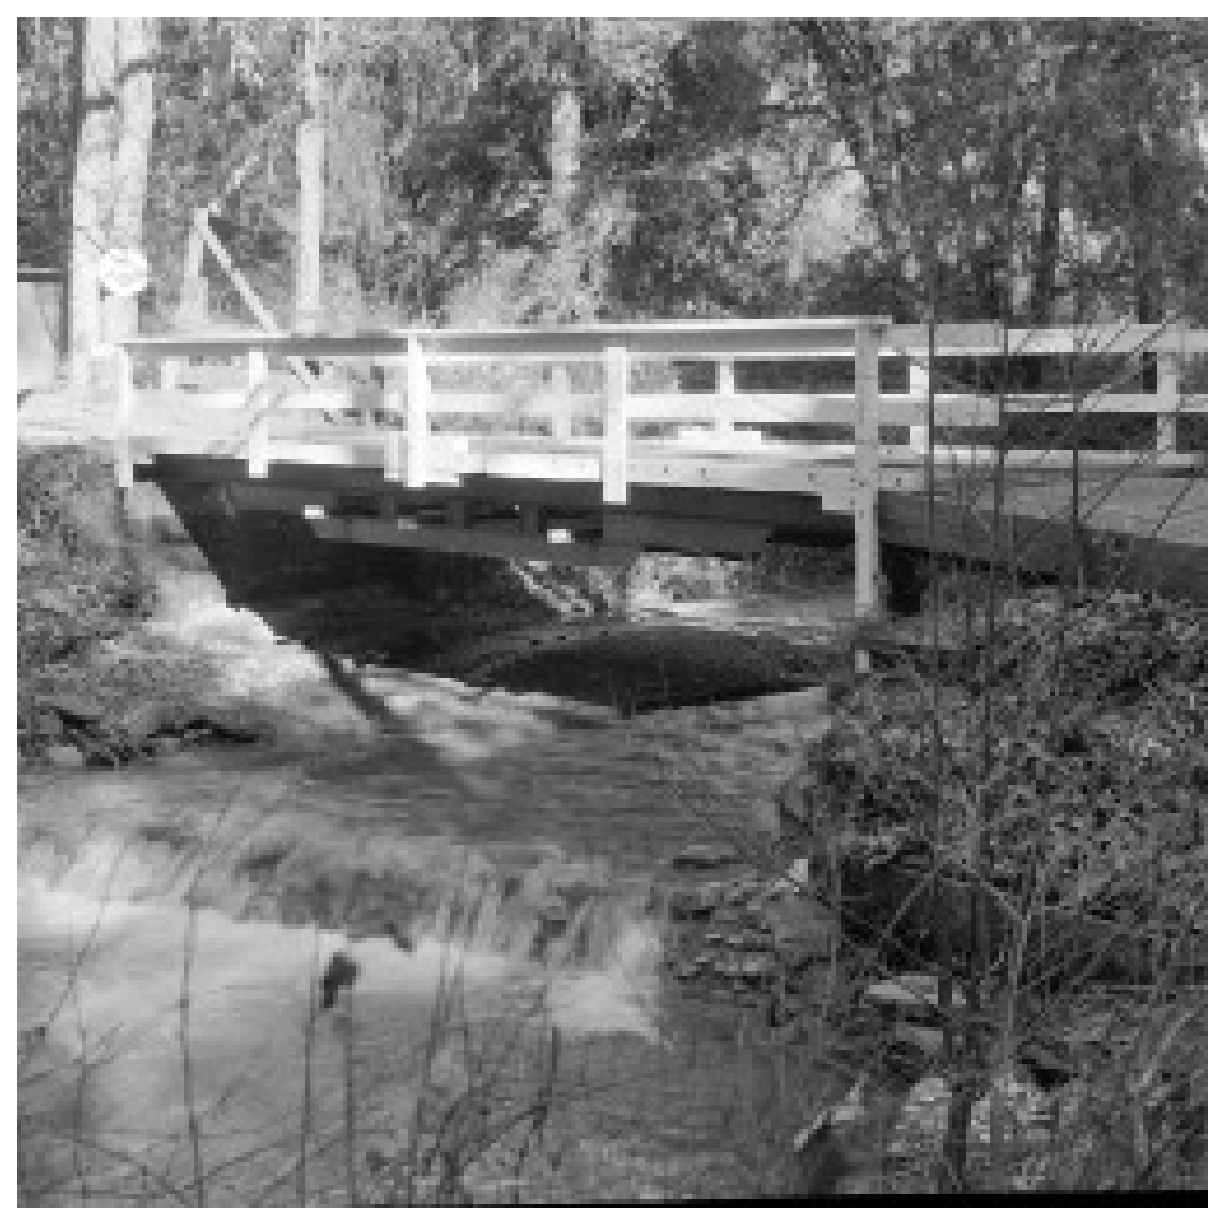
\includegraphics[width=3in]{bridge.eps}
    \caption{The ``Bridge'' image}
    \label{fig:1}
\end{figure}
\end{verbatim}
\begin{figure}[h]
    \centering
    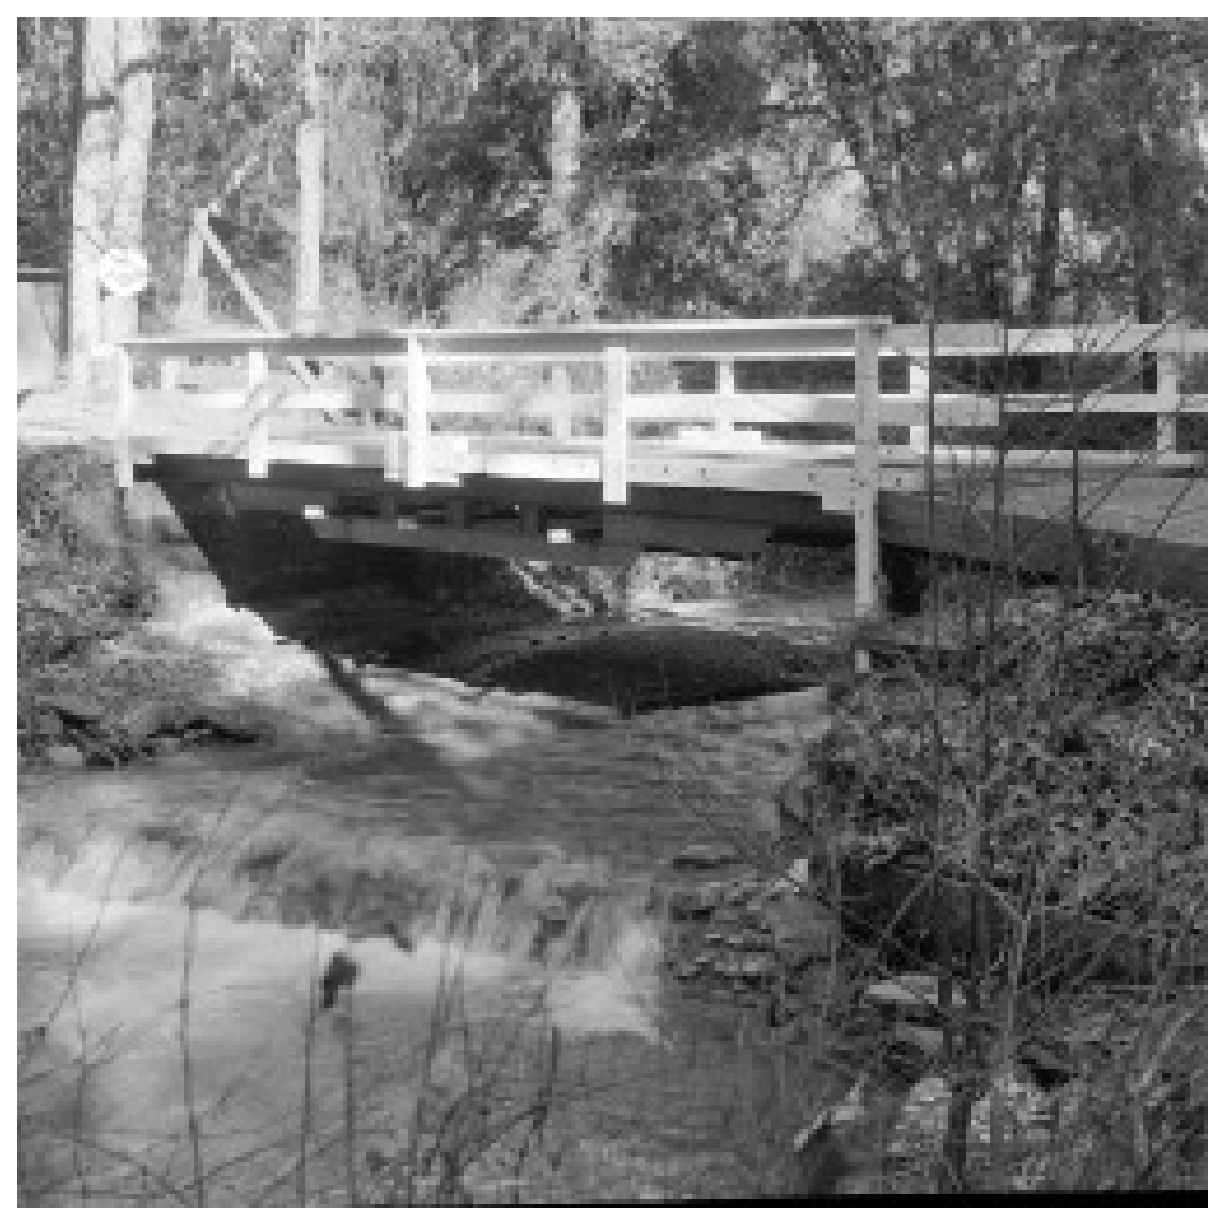
\includegraphics[width=4in]{bridge.eps}
    \caption{The ``Bridge'' image}
    \label{fig:1}
\end{figure}
\texttt{bridge.eps} is a postscript file converted from an image file.
Note that figure \ref{fig:1} is also labeled and cross-referenced here.
For more details about graphics file inclusion, please refer to
\texttt{graphics} package of \LaTeXe.  \LaTeXe\ has a few commands to draw
simple pictures.  Figure \ref{fig:2} shows a picture drawn with \LaTeXe\
commands in the \texttt{picture} environment.  The user can read
\cite{lp:latex} for details.

\begin{figure}
  \centering
\unitlength 0.8in	     % make unit length to be 0.8 inch
\begin{picture}(6,4)(0,0)    % picture coordinates 6 in width, 4 in height,
			     % origin 0,0
\put(1.4,2.6){\line(3,-1){3.0}}   % draw a straight line at slope -1/3
				  % starting at (1.4,2.6) of length 3.0
\put(0,0){\vector(1,0){5.5}}
\put(0,0){\vector(0,1){3}}
\end{picture}

\caption{A Picture Drawn with \LaTeX\ Commands}\label{fig:2}
\end{figure}

\section{Tables-Inserting and Drawing}
Tables and figures are inserted labeled and so on in rather similar ways
except the caption for a table usually appears on top of the table instead
of below that. An example of table is given in Table~\ref{tab:1}. Note
also that this table is written in \textbf{minipage} environment.

\begin{table}
\begin{minipage}[t]{6in}
\caption{Text Formatting and Word Processing Packages}\label{tab:1}
\begin{center}
\begin{tabular}{|l|l|l|}  \hline
	    & Scribe \\ \cline{2-2}
	    & \TeX   \\ \cline{2-2}
Text Formatters\footnote{All the text formatters listed are command-driven}%
	    & \LaTeX \\ \cline{2-2}
	    & troff  \\ \hline
	    & WordStar \\ \cline{2-2}
Word processors \footnote{All the word processors listed are menu-driven}%
	    & Word Perfect  \\ \cline{2-2}
	    & Ms Word	\\ \cline{2-2}
	    & MacWrite	\\ \hline
\end{tabular}
\end{center}
\end{minipage}
\end{table}
Note also that Table~\ref{tab:1} is labeled and referenced. It will be
listed in the LIST OF TABLES.


%%--------------------------------------------------------------------------
\chapter{SPECIAL SYMBOLS}
%%--------------------------------------------------------------------------

\TeX\ has pre-defined many useful special symbols, such as the Greek
letters, mathematical symbols, accented European letters. The newer
version of \TeX\ has even introduced some sets of fonts for some foreign
languages.
For a thesis writer, the most essential knowledge he needs about the
special symbols is Greek letters and mathematical symbols.

\section{Greek Letters}
In \TeX\ and \LaTeXe\ Greek letters are called by  their English names,
e.g., alpha, beta. If the first letter is in capital, then \TeX\ outputs
a capital Greek letter (but many capital Greek letters coincide with
English letters, and hence no commands are designed for them).
The commands for all the Greek letters are listed in
Table \ref{tab:greek}. Note that Greek letters have to be in math mode,
e.g., $\alpha$.

\section{Other Mathematical Symbols}
Beside the Greek letters there are many more math symbols, for example
the Calligraphic letter $\cal F$ which may used for Fourier and
$\cal L$ for Laplace. The user can refer to the \LaTeXe\ Manual\cite{lp:latex}
pp. 41--50 for more information.  Many mathematical
symbols are listed in Appendix \ref{sec:mathsym}.

\section{Accented European Letters}
In the \LaTeXe\ Manual\cite{lp:latex} pp. 38--39, one can find some help as
for how typeset accented European letters.


